\documentclass[12pt]{article}

\usepackage[french]{babel}
\usepackage{fancyhdr}
\usepackage{amsmath}
\usepackage{amsfonts}
\usepackage[final]{graphicx}
\usepackage{color}
\usepackage{indentfirst}
\usepackage[T1]{fontenc}
\usepackage[justification=centering]{caption}
\usepackage{subcaption}
\usepackage{perpage}
\usepackage{hyperref}
\usepackage{float}
\usepackage[bottom]{footmisc}
\usepackage[a4paper, left=1.2in, right=1.2in, top=1in, bottom=2in]{geometry}
\usepackage{colortbl}
\usepackage{xcolor}
\usepackage[normalem]{ulem}
\usepackage{array}
\useunder{\uline}{\ul}{}

\title{Rapport de projet \\ \textbf{Robot ramasseur de balles de tennis}}
\author{Paul BARBARIN, Mohammed KHERRARZ, Antton CATTARIN}
\date{1A - 2023}

\thispagestyle{plain}

\begin{document}

    \begin{titlepage}

        \begin{figure*}
            \centering
            
\includegraphics{img/enseirb}
        \end{figure*}
        \maketitle

    \end{titlepage}

    \tableofcontents
    \pagebreak
    
    \section{Introduction}
    \label{sec:intro}

    L'objectif de ce projet est de travailler sur différentes méthodes algorithmiques. Selon cet objectif, nous déterminerons une solution permettant à un robot de ramasser un certain nombre de balles de tennis disposées sur un terrain, lui aussi, d'une certaine dimension.

    Le cours de théorie des graphes prend alors tout son sens, ces mêmes-balles pouvant être représentées comme des sommets. Nous tenterons, dans ce rapport, d'apporter une solution à ce problème, ce dernier se rapprochant étroitement du problème de celui du voyageur de commerce.
    Quelques spécificités viennent cependant s'y ajouter. En effet, le robot est caractérisé par une vitesse de rotation, supplémentant la vitesse de déplacement. Cette particularité est nécessaire puisqu'elle intervient lorsque le robot doit effectuer une rotation pour continuer son parcours.

    Dans un premier temps, nous mettrons en avant et justifierons nos choix de modélisation du problème. Nous discuterons ensuite de la manière d'implémenter ces choix de modélisation en python. Puis, nous rentrerons dans la majeure partie du projet ; nous présenterons deux de nos solutions algorithmiques, pour ensuite les mettre en confrontation. Nous parlerons des inconvénients de chacunes d'elles, ainsi que de leurs avantages.

    \section{Choix de modélisation et implémentation}
    \label{sec:model_impl}

    Nous avons choisi d'implémenter le graphe par une matrice d'adjacence de dimension 3. Plus précisément, en considérant la rotation que le robot doit effectuer pour aller d'une balle à une autre en provenant d'une tierce, notre matrice d'ajacence possède les 3 dimensions suivantes :

    \begin{itemize}
        \item Dimension 1 : Sommet précédent (Dernier sommet visité par le robot). Ce sommet présente une très grande importance, car il indique de quel chemin vient le robot et donc par extension son orientation (direction),
        \item Dimension 2 : Sommet courant (Sommet actuellement visité par le robot),
        \item Dimension 3 : Sommet suivant (Sommet suivant à visiter par le robot).
    \end{itemize}

    Cette implémentation du graphe par une matrice d'adjacence en 3 dimensions permet ainsi de représenter le poids, mais également et surtout l'angle entre 3 sommets du graphe. Nous pourrons alors considérer cela dans le calcul du temps de parcours. Un exemple simple est présenté ci-dessous :

    \begin{figure}[H]
        \centering
        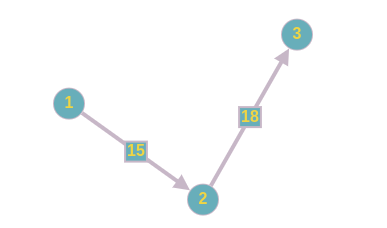
\includegraphics[scale=0.7]{img/example_3dim}
        \caption{3 sommets liés d'un graphe}
        \label{img_3somlinked}
    \end{figure}

    Ici, si $M$ est notre matrice d'adjacence, la valeur $M[1][2][3]$ sera égale au temps que mettra le robot à ramasser la balle 3, en sachant qu'il se situe actuellement sur la balle 2 et qu'il vient de ramasser la balle 1. Cette dernière information nous indique qu'il faut prendre en compte le fait que le robot doit effectuer une rotation de $90$° vers la gauche.

    \section{Deux approches différentes}
    \label{sec:diff_approch}
    
    Pour répondre au sujet, deux algorithmes ont été mis en place. Le premier, lent, cherchant à calculer le chemin optimal, et le deuxième, plus rapide, donnant une solution proche de l'optimale.

    \subsection{Trouver la solution optimale, algorithme naïf}
    \label{subsec:sol_opti}

    Notre algoritme, permettant de calculer le chemin le plus court, explore tout le chemins possibles et retourne le plus court. Pour ce faire, nous avons utilisé la fonction \verb|permutations()| du module \verb|itertools| afin d'obtenir un itérable de toutes les permutations de balles possibles. Chaque permutation correspond à un chemin possible. La complexité de cette fonction est en $O(n!)$, avec $n$ le nombre de balles.

    Ensuite, pour chaque permutation obtenue, l'algorithme calcule le poids total du chemin. Il cherche donc $n$ fois le poids correspondant au déplacement voulu dans la matrice d'adjacence. L'avantage de l'avoir définie telle qu'indiquée dans la partie \ref{sec:model_impl} se ressent ici puisque ces opérations se font en temps constant. Comme nous avons $n$ balles, et $n!$ permutations, trouver le chemin le plus court parmi toutes les permutations se fait en $O(n.n!) = O(n!)$.

    Finalement, cet algorithme a une complexité factorielle, tout comme la résolution du problème du voyageur de commerce selon un approche naïve. Il faut donc s'attendre à ce que le temps de calcul augmente très vite au fur et à mesure que nous ajouterons des balles au problèmes.

    Afin de réduire le nombre d'opérations réalisées, l'algorithme passe à la permutation suivante si le poids de celle en cours excède le poids minimum des chemins précédemment parcourus (même si toutes les balles ne sont pas encore atteintes).

    \subsection{Approximer la solution, algorithme de proche en proche}
    \label{subsec:sol_approch}

    L'algorithme cherchant à calculer une solution se rapprochant du chemin l'optimal a une compléxité nettement inférieure au précédent. En effet, son fonctionnement induit une grande baisse des opérations.

    Le programme, à chaque nouvelle position, calcule la balle la plus proche en allant chercher les informations nécessaire dans la matrice. Pour chaque nouvelle balle ramassée, la précédente ne sera pas prise en compte dans le calcul.

    Toujours avec $n$ le nombre de balle, si on se trouve à la $i$ème balle ($0\leq i<n$), l'algorithme calculera le poids de $n-i$ balles.
    
    Au total, il effectuera $\sum_{i=0}^{n}(n-i) = n^2 - \sum_{i=0}^{n}i = n^2 - \frac{n^2 - n}{2} = \frac{n^2 + n}{2}$ opérations. Autrement dit, l'algorithme en une complexité en $O(n^2)$.

    \section{Résultats}
    \label{sec:result}

    Nous avons fait tourner nos algorithmes sur de nombreux jeux de tests. Afin de mesurer le temps pris par ces derniers, nous avons fait varier le nombre de balles, ainsi que les vitesses de rotation et de déplacement du robot. Nous nous attendions à observer des comportements différents.

    La figure \ref{fig:timepathopt} montre le temps d'exécution des deux algorithmes (en échelle logarithmique) selon le nombre total de balles à ramasser. 

    \begin{figure}[H]
        \centering
        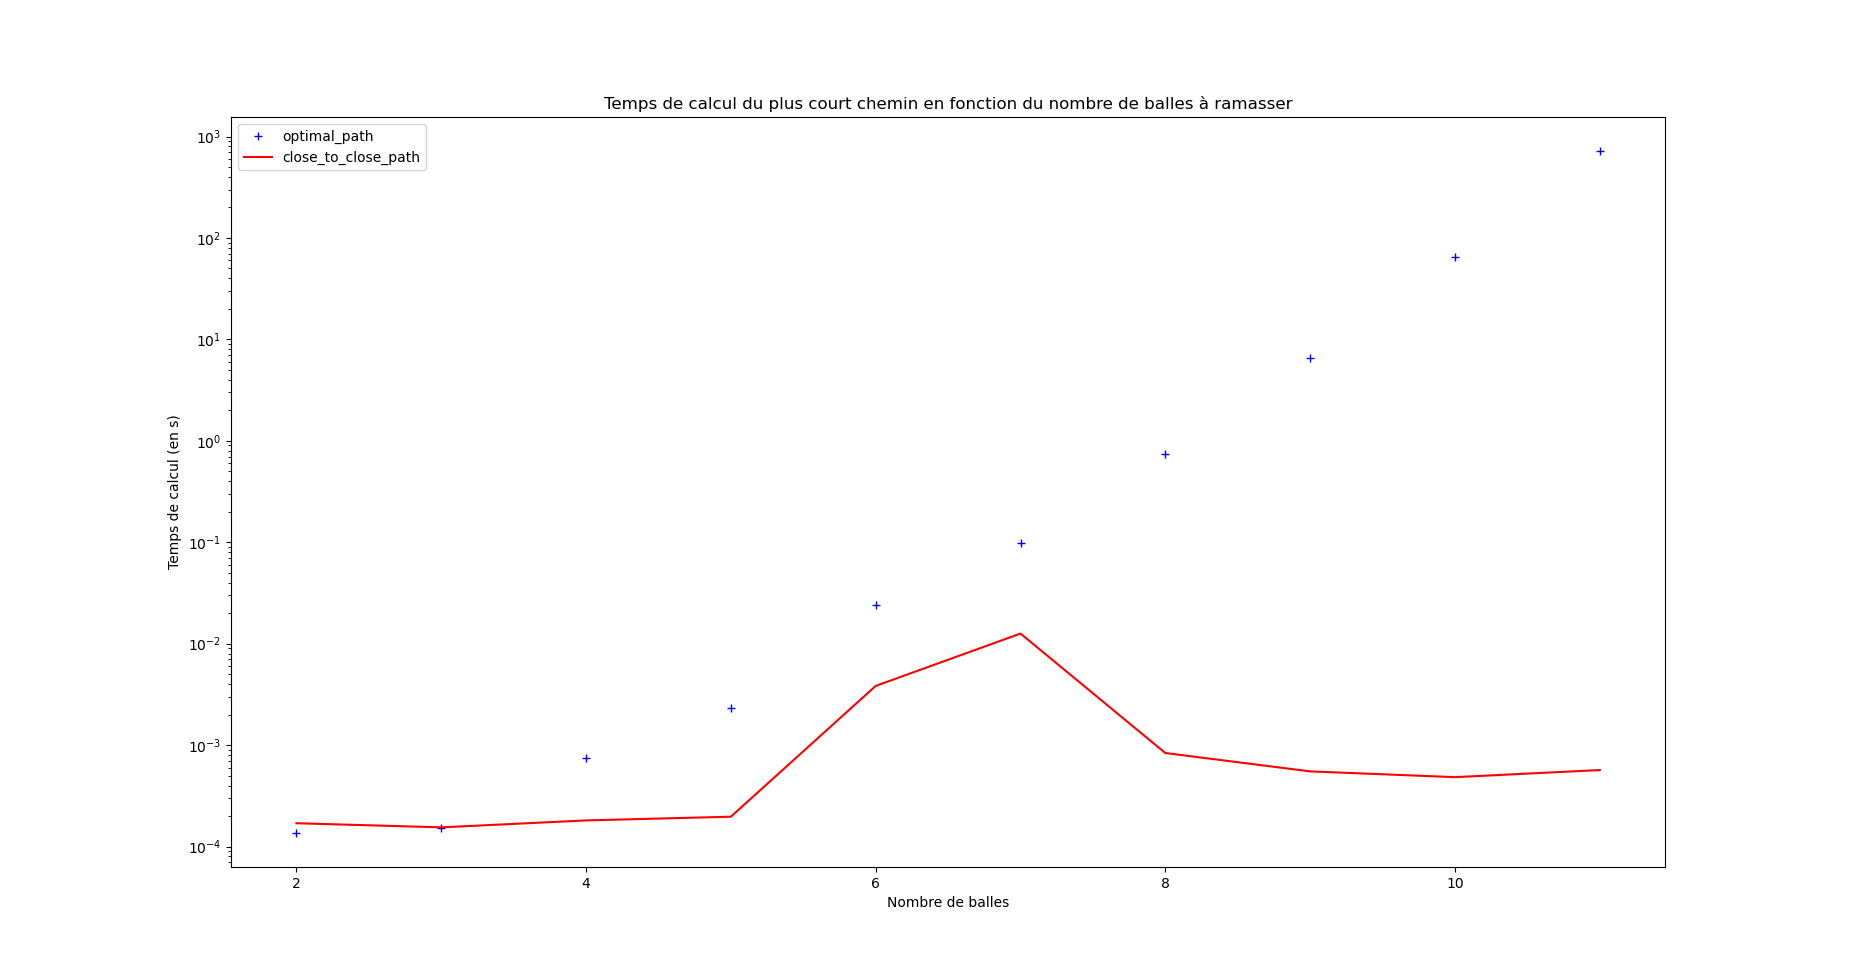
\includegraphics[width=\textwidth]{img/time_path_opt}
        \caption{Temps de calcul des deux algorithmes en fonction de nombre de balles à ramasser}
        \label{fig:timepathopt}
    \end{figure}

    Nous remarquons bien que le temps de calcul augmente considérablement pour l'algorithme naïf lorsqu'on rajoute une balle au monde, tandis que l'algorithme de proche en proche augmente beaucoup moins rapidement. Pour le premier algorithme, le temps pris est de 10 secondes pour 9 balles, et presque de 15 minutes pour 11 balles. Ceci nous montre bien les limites de ce genre d'algorithme, qui sont que, pour des problèmes de grande taille, le temps de calcul devient rapidement trop important. Cela est bien en adéquation avec notre étude de la complexité de cet algorithme.

    La figure \ref{fig:timemoreballs} montre le temps d'exécution de l'algorithme de proche en proche, pour des nombres de balles plus importants

    \begin{figure}[H]
      \centering
      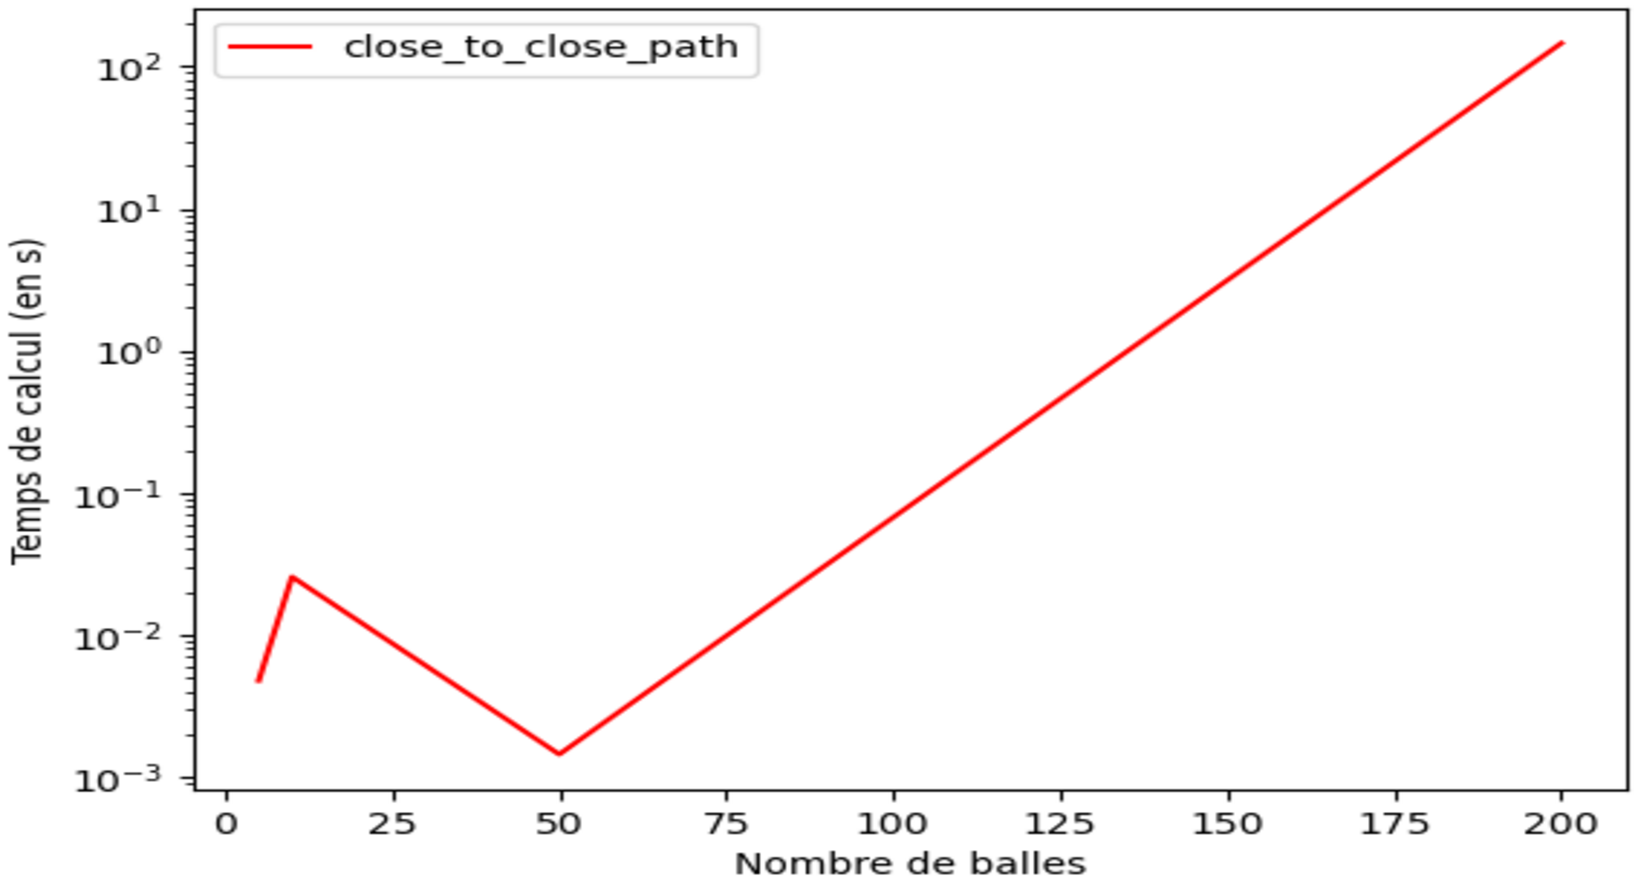
\includegraphics[width=\textwidth]{img/time_more_balls}
      \caption{Temps de calcul de l'algorithme de proche en proche pour des nombres de balles plus important}
      \label{fig:timemoreballs}
  \end{figure}

    Le temps de calcul pour 200 balles avec cet algorithme est approximativement égal au temps pris pour 10 balles par l'algorithme naïf. Il est important de noter que ces valeurs dépendent fortement de la machine sur laquelle sont effectués les opérations. La tendance générale reste malgré tout la même.
    Le test a aussi été fait pour 1000 balles, mais le temps d'initialisation du graphe devenait trop important. En effet, elle se fait en $O(n^3)$ (matrice en 3 dimensions), et a même une complexité plus importante que l'algorithme de proche en proche. 
    
    \medskip
    
    Ensuite, nous avons utilisé les algorithmes dans plusieurs mondes différents, en faisant varier les vitesses du robot. Lorsque la vitesse de déplacement était faible devant la vitesse de rotation, nous nous attendions à avoir un chemin minimisant la distance parcourue par le robot. A l'inverse, lorsque la vitesse de rotation était la plus faible, nous nous attendions à un chemin minimisant les angles lors du déplacement, c'est à dire un chemin le plus circulaire possible.

    Les figures \ref{subfig:terrain3od} (resp. \ref{subfig:terrain3or}) donne le chemin le plus court obtenu lorsque la vitesse de déplacement (resp. de rotation) était plus grande que la vitesse de rotation (resp. de déplacement). L'étoile verte marque la position initiale du robot, tandis que le croix rouge représente la première balle ramassée.

    \begin{figure}[H]
        \centering
        \begin{subfigure}{0.35\textwidth}
          \centering
          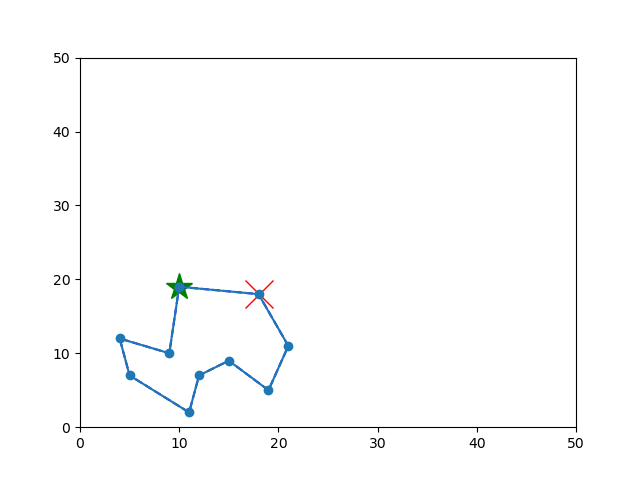
\includegraphics[width=\linewidth]{img/3od}
          \caption{Vitesse de déplacement ($v_d$) $<<<$ vitesse de rotation ($v_r$)}
          \label{subfig:terrain3od}
        \end{subfigure}
        \hfill
        \begin{subfigure}{0.35\textwidth}
          \centering
          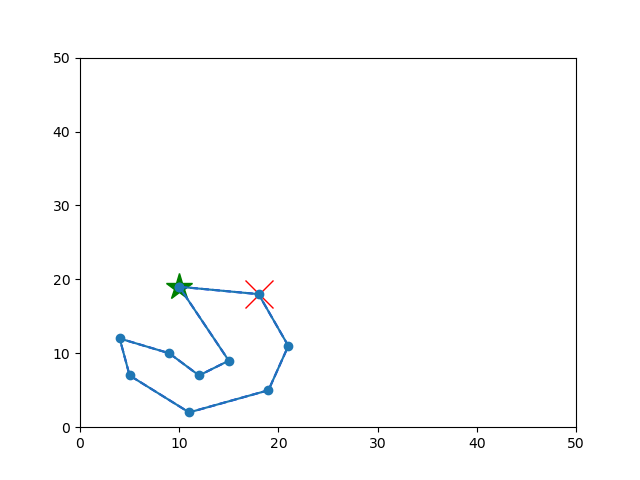
\includegraphics[width=\linewidth]{img/3or}
          \caption{$v_r$ $<<<$ $v_d$}
          \label{subfig:terrain3or}
        \end{subfigure}
        \caption{Chemins optimaux obtenus avec l'algorithme naïf}
        \label{fig:terrain3opt}
    \end{figure}

    Les chemins obtenus sont en adéquation avec les résultats attendus.

    \medskip

    En comparaison, voici en figure \ref{fig:terrain3close} les chemins obtenus avec le second algortihme :

    \begin{figure}[H]
      \centering
      \begin{subfigure}{0.35\textwidth}
        \centering
        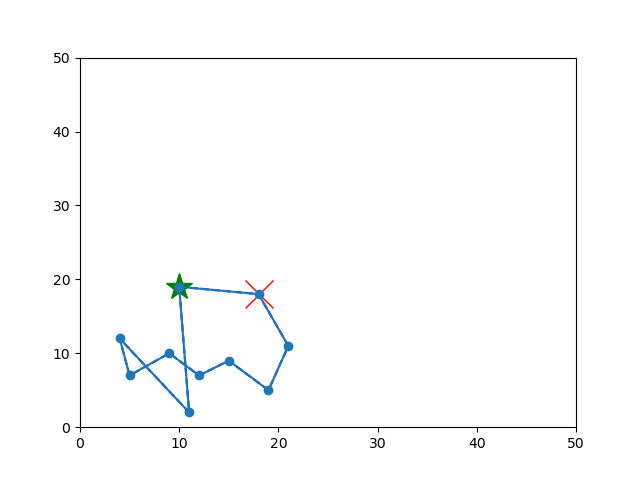
\includegraphics[width=\linewidth]{img/3cd}
        \caption{$v_d$ $<<<$ $v_r$}
        \label{subfig:terrain3cd}
      \end{subfigure}
      \hfill
      \begin{subfigure}{0.35\textwidth}
        \centering
        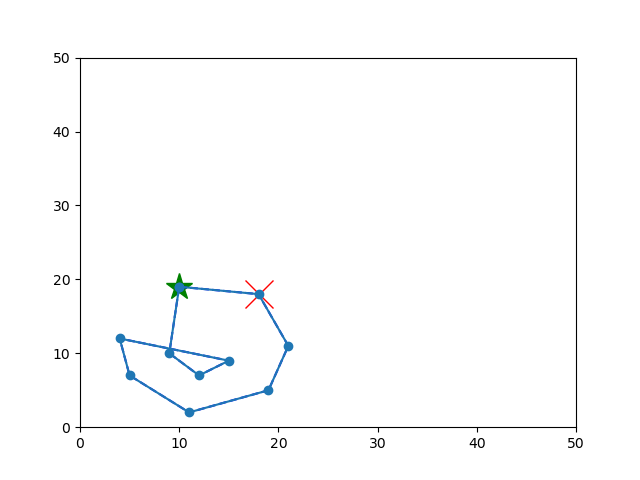
\includegraphics[width=\linewidth]{img/3cr}
        \caption{$v_r$ $<<<$ $v_d$}
        \label{subfig:terrain3cr}
      \end{subfigure}
      \caption{Chemins obtenus avec l'algorithme de proche en proche}
      \label{fig:terrain3close}
  \end{figure}

    \medskip

    Un exemple encore plus parlant est celui du monde fourni dans le sujet du projet. Dans les deux conditions énoncées précédemment, nous obtenons la figure \ref{fig:terrain2opt} :

    \begin{figure}[H]
        \centering
        \begin{subfigure}{0.35\textwidth}
          \centering
          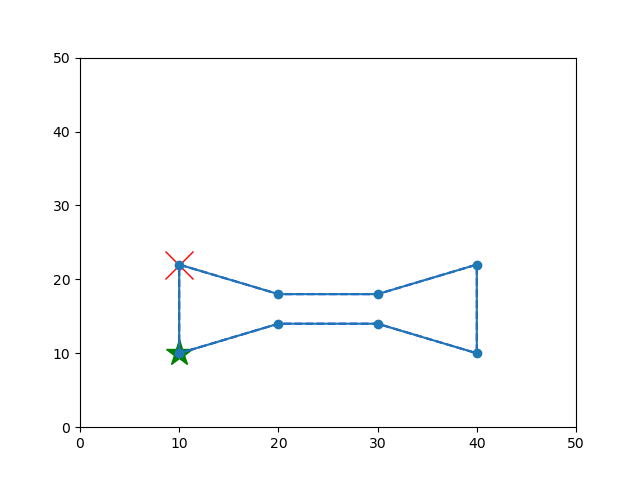
\includegraphics[width=\linewidth]{img/2od}
          \caption{$v_d$ $<<<$ $v_r$}
          \label{subfig:terrain2od}
        \end{subfigure}
        \hfill
        \begin{subfigure}{0.35\textwidth}
          \centering
          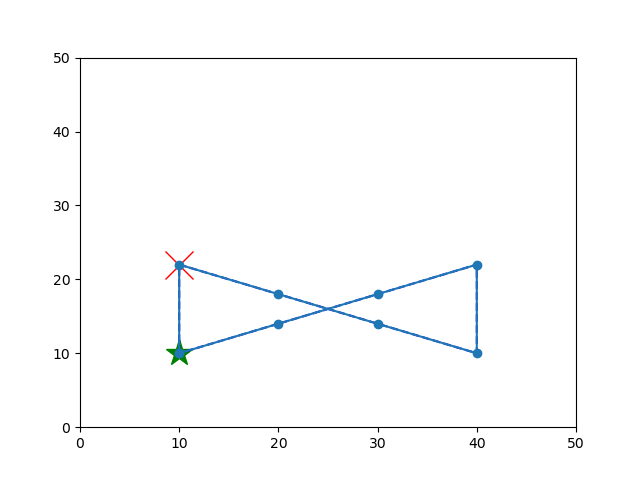
\includegraphics[width=\linewidth]{img/2or}
          \caption{$v_r$ $<<<$ $v_d$}
          \label{subfig:terrain2or}
        \end{subfigure}
        \caption{Chemins optimaux obtenus avec l'algorithme naïf}
        \label{fig:terrain2opt}
    \end{figure}

    Nous pouvons remarquer que les chemins reliant les 4 sommets de la partie gauche est identique dans les deux situations (idem pour les 4 sommets de la partie droite). La seule différence se trouve au milieu.

    Il est facile de voir que la distance parcourue est plus petite dans la figure \ref{subfig:terrain2od}, tandis que les angles sont réduits au maximum dans la figure \ref{subfig:terrain2or} (plus de lignes droites).

    Les chemins calculés par l'algorithme de proche en proche sont présents en figure \ref{fig:terrain2close}.

    \begin{figure}[H]
      \centering
      \begin{subfigure}{0.35\textwidth}
        \centering
        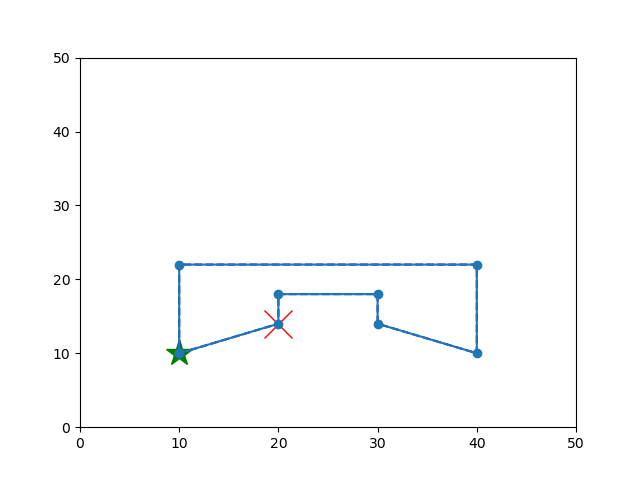
\includegraphics[width=\linewidth]{img/2cd}
        \caption{$v_d$ $<<<$ $v_r$}
        \label{subfig:terrain3mvt}
      \end{subfigure}
      \hfill
      \begin{subfigure}{0.35\textwidth}
        \centering
        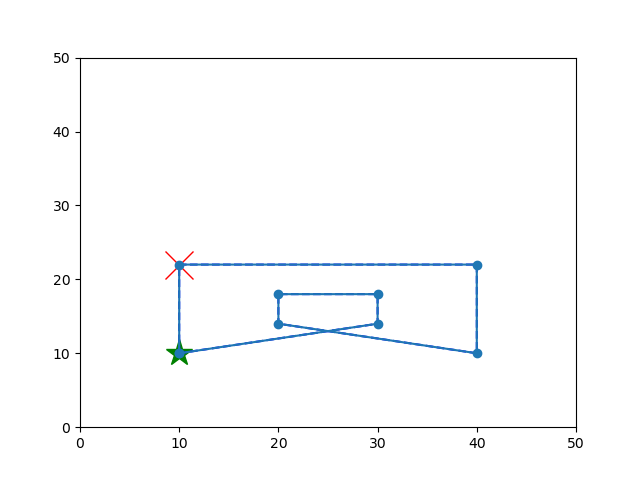
\includegraphics[width=\linewidth]{img/2cr}
        \caption{$v_r$ $<<<$ $v_d$}
        \label{subfig:terrain3rot}
      \end{subfigure}
      \caption{Chemins obtenus avec l'algorithme de proche en proche}
      \label{fig:terrain2close}
    \end{figure}

    \bigskip

    La taille du monde, elle, n'a aucun impact sur les résultats. En effet, les sommets de notre graphe sont uniquement les balles à ramasser, donc la taille totale du monde n'a aucune incidence (sauf s'il devient trop petit et donc que certaines balles ne soient pas à considérer).

    Les algorithmes ont également été essayé sur un autre monde plus petit. Les résultats sont présents en figure \ref{fig:terrain1opt} et \ref{fig:terrain1close}.

    \begin{figure}[H]
      \centering
      \begin{subfigure}{0.35\textwidth}
        \centering
        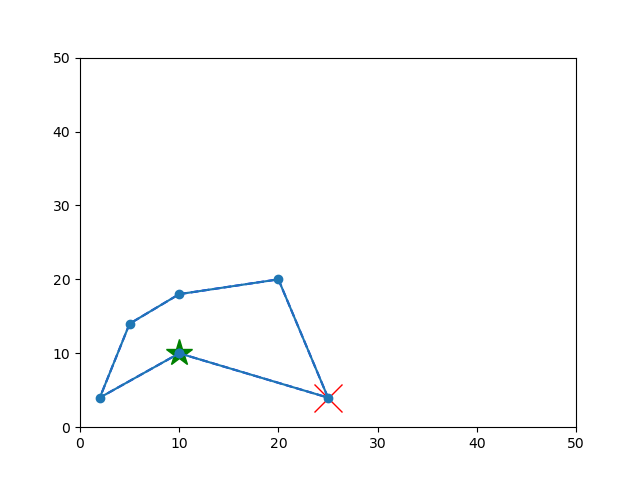
\includegraphics[width=\linewidth]{img/1od}
        \caption{$v_d$ $<<<$ $v_r$}
        \label{subfig:terrain3mvt}
      \end{subfigure}
      \hfill
      \begin{subfigure}{0.35\textwidth}
        \centering
        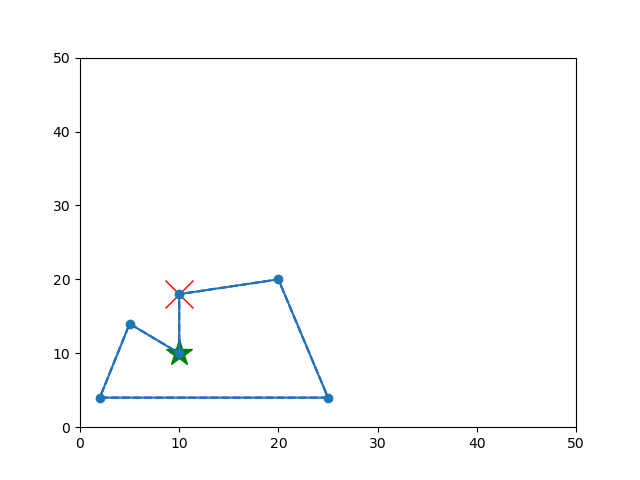
\includegraphics[width=\linewidth]{img/1or}
        \caption{$v_r$ $<<<$ $v_d$}
        \label{subfig:terrain3rot}
      \end{subfigure}
      \caption{Chemins optimaux obtenus avec l'algorithme naïf}
      \label{fig:terrain1opt}
    \end{figure}

    \begin{figure}[H]
      \centering
      \begin{subfigure}{0.35\textwidth}
        \centering
        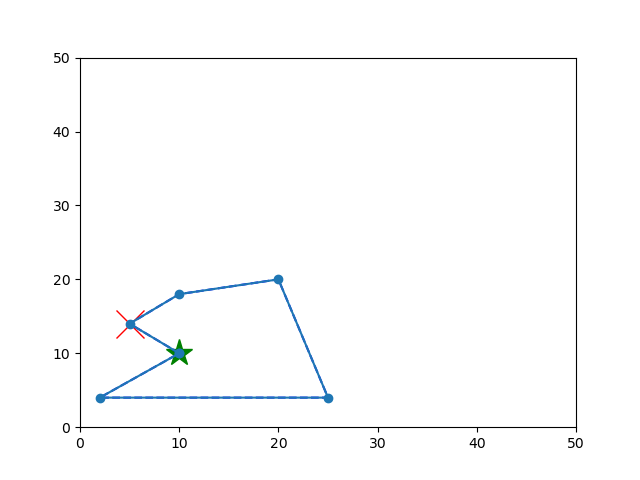
\includegraphics[width=\linewidth]{img/1cd}
        \caption{$v_d$ $<<<$ $v_r$}
        \label{subfig:terrain3mvt}
      \end{subfigure}
      \hfill
      \begin{subfigure}{0.35\textwidth}
        \centering
        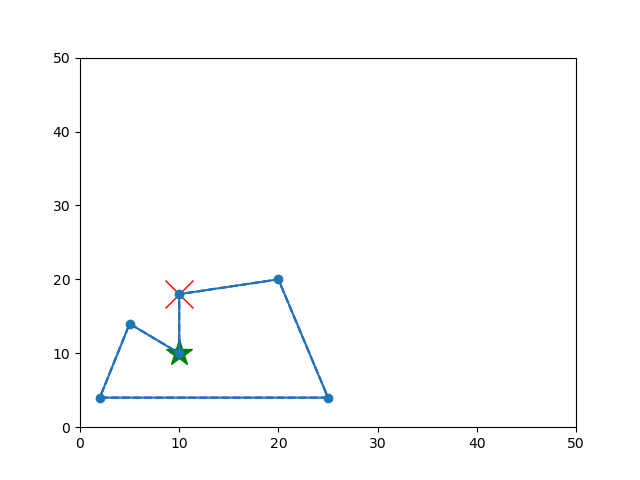
\includegraphics[width=\linewidth]{img/1cr}
        \caption{$v_r$ $<<<$ $v_d$}
        \label{subfig:terrain3rot}
      \end{subfigure}
      \caption{Chemins obtenus avec l'algorithme de proche en proche}
      \label{fig:terrain1close}
    \end{figure}

    Dans tous les essais réalisés, lorsque $v_d <<< v_r$ (resp. $v_r <<< v_d$), on avait $v_d = 0.0001$ et $v_r = 1000$ (resp. $v_r = 0.0001$ et $v_d = 1000$). Les poids des chemins obtenus dans les situations précédentes sont présents dans le tableau suivant :
    
    \medskip
    
    \begin{tabular}{c|c|c|c|c|}
      \cline{2-5}
      & \multicolumn{2}{c|}{$v_d <<< v_r$} & \multicolumn{2}{c|}{$v_r <<< v_d$} \\
      \cline{2-5}
      & naïf & proche & naïf & proche \\
      \hline
      terrain 1 & 870813 & 935400 & 58539 & 107981 \\
      \hline
      terrain 2 & 637138 & 748426 & 114592 & 126770 \\
      \hline
      terrain 3 & 699600 & 727673 & 85287 & 85287 \\
   \end{tabular}

   Les terrains sont numérotés par ordre d'apparition dans le rapport. Nos résultats montrent que le poids total du chemin obtenu et systématiquement inférieur pour l'algorithme naïf. L'autre élément encourageant est que les poids obtenus par l'algorithme de proche en proche est très proche du chemin optimal, voire égal dans un cas. Cependant, dans un autre cas, il y a presque une différence de 100\% entre les deux chemins, ce qui reste tout de même acceptable.

   \section{Conclusion}
   \label{sec:ccl}

   Les deux algorithmes implémentés se sont avérés concluant dans le calcul d'un chemin le plus court possible permettant de résoudre le problème.
   
   Le premier possède un avantage très important : il calcule le chemin le plus court. Cependant, sa compléxité exponentielle le rend difficile, voire impossible d'utilisation lorsuq'il y a plus de 11 balles dans le monde.
   
   Le deuxième, lui, bien qu'il peut paraître simple, parvient à trouver des chemins se rapprochant beaucoup des chemins optimaux. De plus, sa complexité étant relativement faible, au vu du problème considéré, il peut être utilisé avec un nombre de balle pouvant être très grand (au moins 200).

   Finalement, le choix d'implémentation du graphe via une matrice d'adjacence a permis de diminuer la complexité. En effet, le graphe n'a pas besoin d'être modifié à chaque nouvelle position afin d'adapter de temps de rotation du robot. Cependant, lorsque le nombre de balles devient trop important (autour de 1000), la création de la matrice est bien trop longue pour pouvoir exploiter l'algorithme de proche en proche.

\end{document}